%!TEX root = ../document.tex
\chapter{个性化推荐、序列感知推荐及迁移学习}
\section{推荐系统}
推荐系统的定义和概念很多,但1997年Resnick和Varian给出的定义%
被广泛接受,既“推荐系统是利用电子商务网站向客户提供商品信息%
和建议,帮助用户决定应该购买什么产品,模拟销售人员帮助客户%
完成购买过程”。%

通用的推荐系统模型如图\ref{fig:frame}所示,图中%
可以清晰看到,%
推荐系统中很重要的3个模块分别是:用户建模模块、%
推荐对象建模模块推荐算法模块,它通过匹配用户模型%
中兴趣需求信息和推荐对象模型中的特征信息,%
同时结合使用相关的推荐算法进行筛选,推荐用户可能%
感兴趣的对象\upcite{王国霞}。
\begin{figure}[htbp] % use float package if you want it here
  \centering
  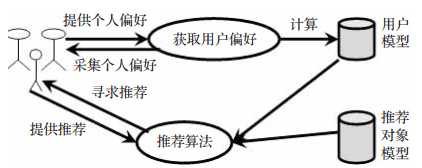
\includegraphics[width=\textwidth]{frame.jpg}
  \caption{推荐系统的通用模型}
  \label{fig:frame}
\end{figure}




\subsection{个性化推荐概述}
个性化推荐能成功,需要具备两个条件,第一是海量的信息,%
因为只有信息量很大的时候用户才需要系统的自动推荐。%
第二是用户没有明确的需求,如果有明确的需求,用户都会选择%
通过浏览器搜索,快速发现感兴趣的东西,而不需要推荐了。%
随着互联网行业的快速发展,信息量的增长速度飞快,%
各种新闻的推送(微博、微信公众号等),占用了很多的时间,%
严重的影响了获取信息的质量问题,%
大量的垃圾信息导致人们获取有价值的信息的成本有所增加,%
并且,人们的生活节奏也日益加快,需要在有限的时间内%
获取对自己有用的信息便难上加难,为了解决信息过载的难题,%
研究人员边通过用户历史行为数据开始对用户兴趣进行建模,从而%
实现个性化推荐的功能,让每个用户都有不一样的个性化页面。%
个性化推荐系统的价值便在于此。%
至今,国内外许多大型的公司投入了大量的精力到推荐系统的研究中,%
因此也给公司带来了很大收益,如最早研究推荐系统的亚马逊。%

在学术社交研究领域个性化人物推荐包括社交好友推荐,%
论文合作作者推荐等。收集用户的历史行为记录,如评分、%
分享、收藏、自定义标签等,通过分析用户的行为,%
给其推荐可能感兴趣的对象,以及用户的个人基本信息,%
如性别、年龄,在推荐系统的研究中,真正难以把握的是用户个性化需求,
\subsection{推荐算法}


\subsection{推荐系统存在的问题}

\textbf{冷启动问题}推荐系统需要数据作为支撑,通常需要根据用户历史行为记录去%
预测未来可能产生的行为和兴趣。现实中,我们面对大量的新用%
户又或者对于全新上线的系统不仅没有有效的用户行为数据而且%
也缺乏用户的个人基本信息(年龄、性别等),我们没有任何数%
据对用户的偏好进行建模,这个问题被称为“冷启动”,是推荐系%
统中面临的一个难题问题。在缺乏用户行为数据的情况下,%
并不是就没办法给用户推荐,
早期的推荐系统会基于商品内容数据做推荐,例如给商品打大%
量的标签或者通过推荐热门商品等方式来%
解决冷启动问题。Yao\upcite{yao2012product}等学者提出%
通过用户搜索的关键字信息去预测用户的偏好,%
具体方式是通过比较搜索的关键词和已有%
的产品的信息做相似性比较,实验证明,他们提出的方法比推荐%
最受欢迎的方法效果更好。

\textbf{噪音问题}大数据时代面临一个很严重的问题,不仅数据量多,而且数据不干净%
要获得高质量的数据往往是不太现实的,需要前期花费人力物力进行%
数据预处理,高效的数据处理能力,能快速的挖掘数据的重要信息。随着需求的提出,研究者们也提出了很多数据处理的%
方式,例如减噪、归一化等。

\textbf{数据长尾问题}个性化推荐系统一开始主要解决的问题就是通过发掘长尾数据来提升%
商家产品的销售额,而长尾商品却仅仅只能代表小部分用户的需求,%
所以只能充分发掘用户的行为,研究用户的兴趣,以此找到用户的个性化需求。%
所以,推荐系统可以更好地发掘数据的长尾。
\section{序列感知模型}
关键词抽取是从文本中提取出重要的短语或词。关键词背%
后所蕴含的丰富信息%
可以高度概括一篇文章的主题信息,该问题一直是自然语言处理中基础问题,也是研究的热点问题,关键词的研究成果被广泛的应用在%
文本分类、聚类、文本摘要、话题监测、索引和搜索等领%
域\upcite{caragea2014citation,常耀2018成关键词提取算法综述,lopez2010humb,bougouin2013topicrank}。%
早于20世纪80年代已经有研究者用TF-IDF进行关键词的抽取。%
随着研究不断的推荐,近年来研究者们不断的提出新的特征或算法,%
如florescu\upcite{florescu2017positionrank}提出计算词出现的平均位置,%
caragea\upcite{caragea2014citation}引入引文的特征等。%
对未来的性能提升方面,常耀成表示可以综合利用现有特征或提出新特征%
\upcite{常耀2018成关键词提取算法综述}。%
赵京胜等人通过从各个维度综述前人的工作后也提出了关键词抽取%
人物未来的发展方向\upcite{赵京胜2017自动关键词抽取研究综述}。%
Hasan\upcite{hasan2014automatic}通过全面调研总结了目前研究%
关键词抽取人物准确率普遍很低的原因,研究者也可以通过解决这%
些存在的问题作为研究思路。%


\subsection{序列感知推荐任务及场景}

当待分析的数据具有固有的顺序性质,序列学习方法就会在这些应用领域中有用,比较常见的应用有如自然语言处理、语音识别、时间序列预测、DNA建模,以及作为本文工作的核心内容,序列感知推荐。


\subsection{序列感知推荐技术分类}

\textbf{频繁集挖掘}

\textbf{马尔可夫链}

\textbf{循环神经网络}
循环神经网络被发明的目的就是用来进行对可变长度的序列数据进行建模。循环神经网络与传统的前馈深度神经网络模型之间的主要区别在于组成网络的单元中存在内部隐藏状态。对于一个标准的循环神经网络其通过以下形式来更新隐藏单元的状态$h$:




\textbf{门控循环单元Gated Recurrent Unit}

\textbf{长短期记忆神经网络}

\textbf{双向循环神经网络}






\subsection{序列感知推荐算法评价指标}



\section{迁移学习}
学术社交网络能为具有共同兴趣的科研工作者提供%
一个实时沟通、共享成果的平台。目前,学术社%
交网络的发展很迅速,其覆盖的面也非常广泛,%
功能也逐渐强大起来,为科研工作者提供很多科%
研社交服务。随着推荐技术的成熟和发展,%
在系统中加入推荐功能成为社交网络的热点,%
可以通过潜在好友关系进行人物推荐,也可以根据相似兴趣%
推荐书籍或论文等。
实时为科研工作者推送一些推荐条目,不仅可%
以节约科研工作者的时间成本,好的用户体验,%
还可以吸引更多的新用户共享研究成果。有相关研究者对国外12个社交网络使用情况进行了调研,参加调研的人中%
超过3000科学家或工程师表示他们知道这些大型的设计网站,但是仅仅只有不到一半的人会定期的去访问ResearchGate。%
详细信息如图\ref{fig:research}所示,%
该图摘自2014年Richard Van Noorden在自然上发表的文章\upcite{van2014online},
从图中可以看出Google Scholar学术社交网站被定期访问的人数是最多的。针对学术社交网站的特殊性%
文中还对用户使用ResearchGate、Academia.edu和Mendeley三个社交平台的日常功能进行了调研,%
详细如下图\ref{fig:three}所示。
国内的社交网站也非常多,例如微博、微信、知乎、百度学术、科研之友、学者网等,但是,本文暂时没有检索到类似的统计相数据。
\begin{figure}[htbp] % use float package if you want it here
  \centering
  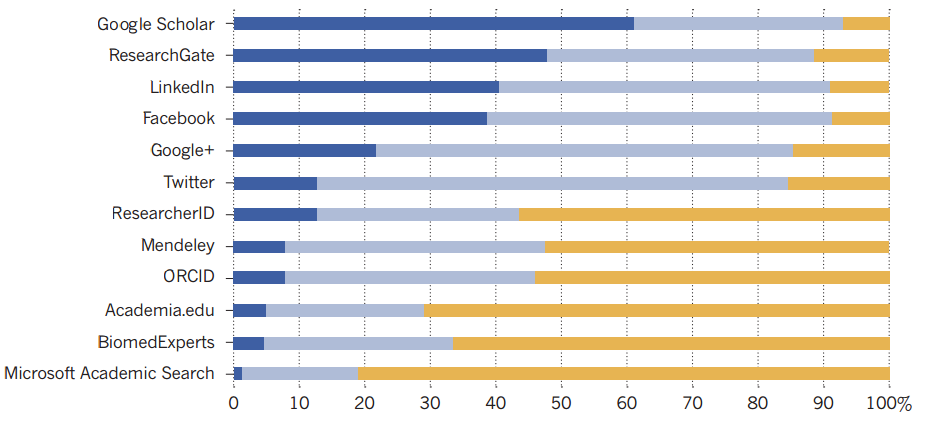
\includegraphics[width=\textwidth]{research.png}
  \caption{国外社交网络使用情况}
  \label{fig:research}
  \footnotesize
  注解:深蓝色表示知道有社交网站并且会定期访问的占比,浅蓝色表示知道有这些社交网站但是不会定期访问%
  的占比,黄色表示不知道有这些科研网站的比例。
\end{figure}
\begin{figure}[htbp] % use float package if you want it here
  \centering
  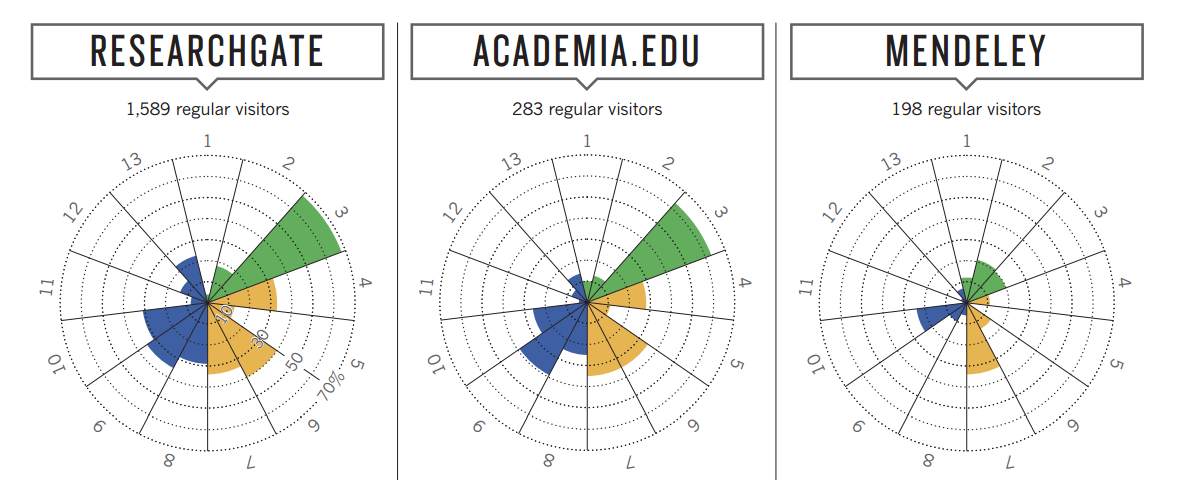
\includegraphics[width=\textwidth]{three.png}
  \caption{调研定期访问学术科研网站的学者的目的}
  \label{fig:three}
  \footnotesize
  注解:1表示不常用,2表示出于好奇,3表示可能有学者联系,4表示追踪指标,5表示找工作,6表示找合作伙伴,%
  7表示查看推荐的论文,8表示联系同行,9表示发布研究内容,10表示分享链接,11表示发起相关研究的讨论,%
  12表示对研究进行评论,13表示跟踪讨论进展;其中有1589位常访问ResearchGate的用户参加了调研,283位%
  参加了Academia.edu调研,198位参加了Mendeley的调研。
\end{figure}

社交网络的发展时间脉络如图,引自\ref{杨雪萍2017科研社交网站中的学者推荐研究}
\begin{figure}[htbp] % use float package if you want it here
  \centering
  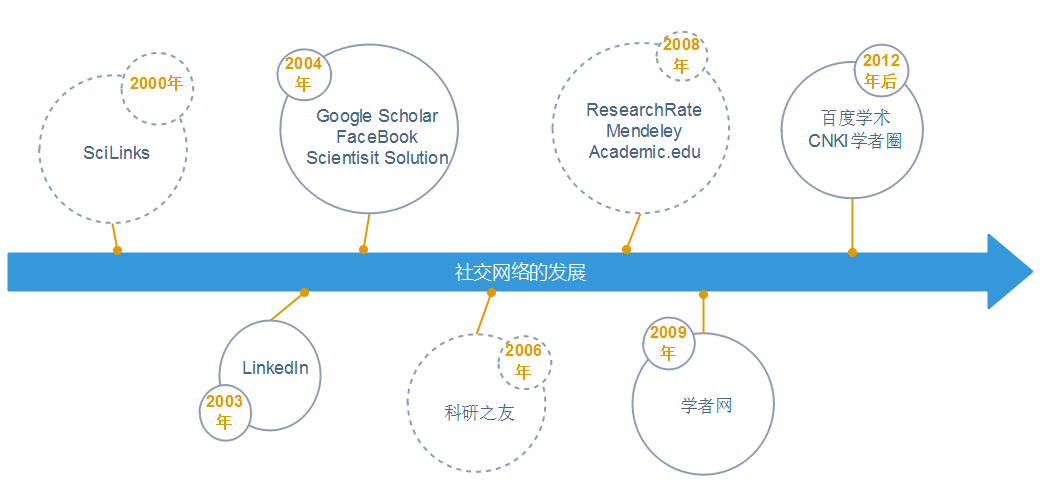
\includegraphics[width=\textwidth]{timeline.jpg}
  \caption{社交网络的发展}
  \label{fig:academic_time}
\end{figure}

为了对比国内外学术社交网络发展的状况,
接下来,本文着重介绍国内外四个知名的科研社交网络平台:%

\textbf{ResearchGate}\footnote{\url{https://www.researchgate.net}}被称为“科学研究的脸书%
(facebook for research)”,%
自2008年上线到现在,该平台的研究者数量已经高达15亿多,包括45名诺贝尔获得者,
学者可以在此网站上分享研究成果、学术论著、并且也可以%
加入一些科研论坛小组。通过注册时填写感兴趣的领域、%
专业知识等信息,其他跟你有相似研究兴趣的科研工作%
者可以很容易发现你。根据个人兴趣,ResearchGate会推荐有相似研究兴趣的研究成果,%
此外,该网站还会根据用户兴趣推荐工作,%

\textbf{Academia.edu}\footnote{\url{https://www.Academia.edu}}于2008创建,截止到2018年12月,%
该网站统计已经有71亿学者加入Academia.edu科研社交网站中,上传了21亿论文,并且每月的访客%
超过40亿,是一个非常庞大的数字。发表在PLOS
ONE上的一篇文章表示,上传到Academia.edu的论文的5年内的引用率可以提高原来的69\%。


\textbf{学者网}\footnote{\url{http://www.scholat.com/}}也%


\textbf{Microsoft Academic}\footnote{\url{https://academic.microsoft.com}}
\textbf{Google Scholar}\footnote{\url{https://academic.microsoft.com}}
\textbf{百度学术}\footnote{\url{https://academic.microsoft.com}}

\subsubsection{迁移学习研究内容}


\subsubsection{迁移学习分类}

\subsubsection{迁移学习方法}

\subsubsection{迁移学习面临的问题}

\section{本章小结}

